
Due to the large amount of electronically-available medical publications stored in databases such as PubMed, there has been an increasing interest in applying text mining and information extraction to the medical literature. 
Those techniques can generate tremendous benefits for both medical research and applications. Among the medical literature mining tasks, medical named entity recognition and normalization are the most fundamental tasks.% and the major developments in this area are usually related to these two.


The goal of medical named entity recognition and normalization is to find the boundaries of mentioning from the medical text and map them onto a controlled vocabulary. State-of-the-art studies have demonstrated the superiority of joint modeling of medical named entity recognition and normalization compared to the pipeline implementation due to mutual benefits between them. There are two main limitations of pipeline models: (1) errors from the recognition tagging cascade into normalization errors, and (2) recognition and normalization are mutually useful to each other, but pipeline models cannot utilize these potential benefits. Joint modeling recognition and normalization can naturally alleviate these %two drawbacks 
limitations and achieve better performance. For example, \citeauthor{Leaman2016TaggerOne} (\citeyear{Leaman2016TaggerOne}) leveraged a joint scoring function for medical named entity recognition and normalization. \citeauthor{Lou2017A} (\citeyear{Lou2017A}) proposed a transition-based model to jointly perform medical named entity recognition and normalization, casting the output construction process into an incremental state transition process. However, these existing joint modeling methods (1) rely heavily on hand-crafted features and task specific resources thus fail to encode complicated and general features such as character-level and semantic-level features; 
(2) use simplistic ways to jointly model medical named entity recognition and normalization, which cannot provide essential mutual supports between these two.   

To improve the joint modeling medical named entity recognition and normalization (MER and MEN), we propose a novel deep neural multi-task learning (MTL) framework with two explicit feedback strategies, which can make use of the mutual benefits between recognition and normalization in a more advanced and intelligent way. First, our method benefits from general representations of both tasks provided by multi-task learning, which enjoys a regularization effect~\cite{Collobert2011,DBLP:journals/corr/Ruder17a} that leads to more general representations to help both tasks. Specifically, it minimizes over-fitting to any specific tasks, thus makes the learned representations universal across tasks. Second, our method can successfully convert hierarchical tasks into a parallel multi-task setting while maintaining mutual supports between tasks. Although the general concept of deep neural multi-task learning is not new, the innovation of our method is that it incorporates both the feedback strategies from the low-level task to the high-level task and vice versa, as shown in Figure~\ref{fig: trans}. 
These two feedback strategies exploit the output of entity recognition to improve entity normalization and vice versa. In addition, our method uses Bi-LSTM to boost the sequential modeling of text and CNN to encode clues hidden in character-level features such as \textbf{Zo}lmitriptan, \textbf{Zomig} and \textbf{Zomig}on.
\begin{figure}[tp]
	\centering
	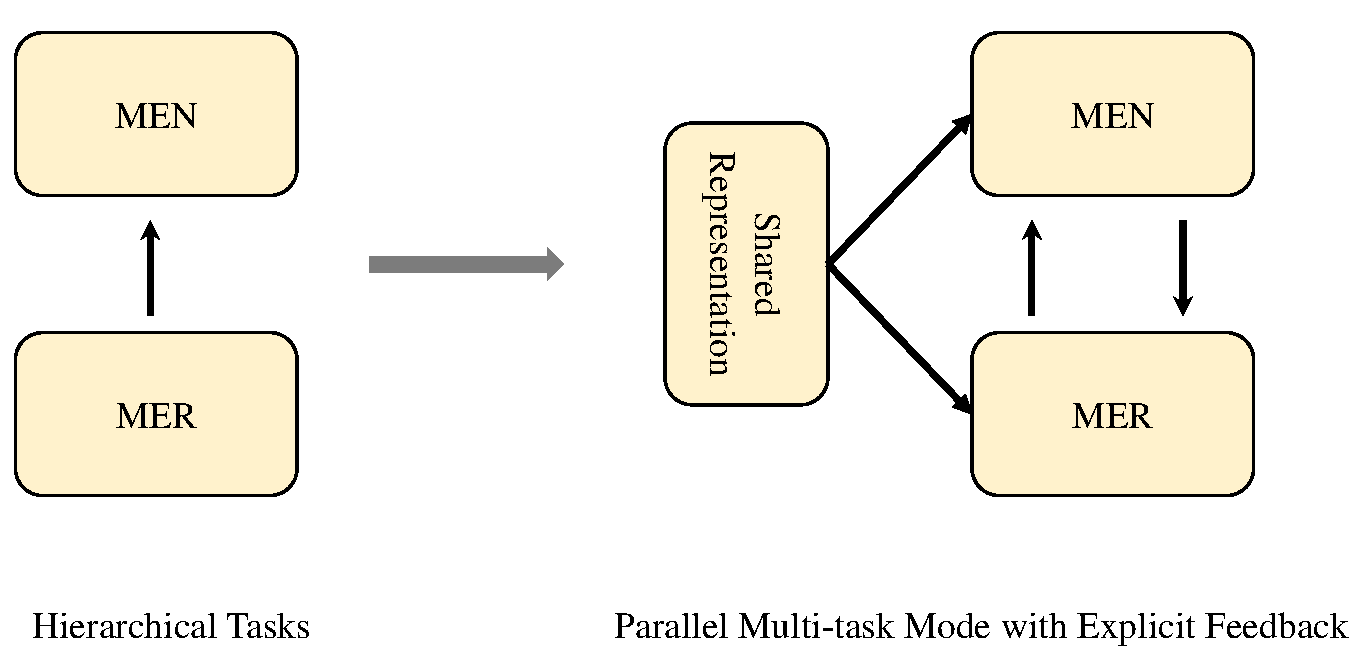
\includegraphics[width=0.4\textwidth]{fig/tranformation}
	\vspace{-0.1in}
	\caption{From hierarchical tasks to parallel multi-task mode by incorporating explicit feedback strategies among tasks. %MER refers to medical named entity recognition, MEN refers to medical named entity normalization.
		}\label{fig: trans}
	\vspace{-0.15in}
\end{figure}

We evaluate our models across two corpora (the BioCreative V Chemical Disease Relation (BC5CDR) task corpus \cite{Li2016BioCreative} and the NCBI Disease corpus \cite{Rezarta2014NCBI}) of medical articles and outperform the state-of-the-art study by up to 4.53\% F1 on medical named entity recognition and 5.61\% F1 on medical named entity normalization.



\noindent\textbf{Contribution.}
To make use of the mutual benefits in a more sophisticated way, we propose a novel deep neural multi-task learning framework with explicit feedback strategies to jointly model named medical entity recognition and normalization. This method incorporates both the feedback strategies from the low-level task to the high-level task and vice versa, which makes it possible to convert hierarchical tasks, i.e. MER and MEN, into parallel multi-task mode while maintaining mutual supports between tasks.
